*The access to a centralized point of storage for experimental data also allows
for real-time continuous logging of various parameters used as indicators for
system health. Critical system parameters can hence be monitored and used to
trigger alarms when these fall out of specified ranges. Furthermore, the
logging of experimental setup parameters continuously enables access to these
values at any previous point in time.

A system design of many highly decentralized clients all pushing data
continuously to a central server requires high server performance, high uptimes
as well as a flexible storage ensuring easy expansion of storage space if
needed. To ensure these properties of the system it has been designed as simple
as possible to avoid unnecessary complications and to ensure that this central
component can be easily managed by the professional IT-staff of the department.
It is important to realize that even though it is typically not a problem if a
single client machine somewhere in the system is temporarily down (this can
happen for many reasons in a experimental lab) it is crucial that the server is
handled like a real production server.

To keep the server side simple we are use a relational database. In our case
MySQL\cite{mysql} database is used which is both open source and provides
extremely good performance. The MySQL server contains the entire set of data
of all experimental setups making it is extremely easy to backup everything by
a dump of the database with regular intervals.

Since the database is only exposed to the local network security is not a real
concern, however, to protect against accidental pollution of the various setups
with irrelevant data when code is exchanged between setups each client has its
own username and password which is not part of the code (typically it will be
managed in the local ODBC-settings of the client). In this way, code can flow
back and forth between setup without the risk of one setup accidentally logging
data to other setup's tables.

\subsection{SQL} The flexible nature of SQL allows one to extract data in many
ways. Complete datasets can be retrieved by simple statements
\begin{verbatim}
 select {*} from table_name
\end{verbatim}

This data can the be handled using the programming environment most comfortable
for users and can be used for instance to perform automatic reporting, data
treatment or as input to scripts that will produce plots based on the data. SQL
also allows for very efficient data treatment directly from the SQL-server
which can be very useful to get a quick overview of the acquired data. As an
example SQL statements can be used to plot the pressure in a vacuum chamber at
1\,A.M. in the morning for the last month. This can be a useful tool to monitor
the general health of the chamber, i.e. if leaks has developed or a valve is
failing
\begin{verbatim}
select unix_timestamp(date(time)), avg(pressure) from pressure_microreactor
where hour(time) = 1 and minute(time) between 00 and 20 and time between
{from} and {to} group by date(time) order by time desc limit 30;
\end{verbatim}
where \{from\}  and \{to\} should be replaced with the relevant time interval.

The output from as a statement like this is illustrated in
Figure~\ref{fig:morning_pressure}.
\begin{figure}
 \begin{center}
 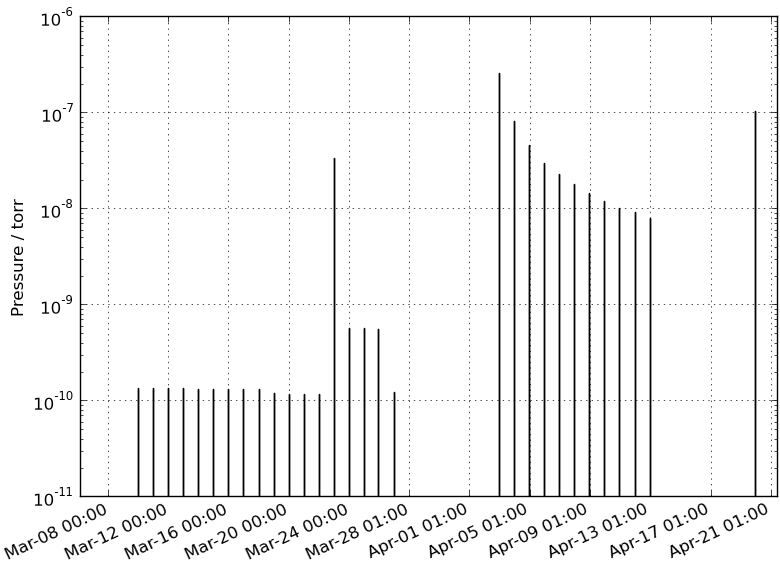
\includegraphics[width=10cm]{morning_pressure.png}
 \caption{ The morning pressure in a vacuum chamber at the department. The
   pressure gauge is unable to read high pressures, and thus no data is
   available from periods where the chamber is vented for maintenance.
   \label{fig:morning_pressure}
 } 
 \end{center}
\end{figure}

A further advantage of SQL servers is the standardization making it rather easy
to change the choice of implementation if this for some reason is wanted.
Several open source implementations of SQL-servers exists.



